% L7b student companion deck.
%
% The frame order mirrors the lecture notebook so students can take notes while
% the instructor works through the notebook. The disclaimer is intentionally
% slide 2, by instructor preference.
\documentclass[aspectratio=169,11pt]{beamer}
\usepackage{vnslides}

\newcommand{\E}{\mathbb{E}}
\newcommand{\R}{\mathbb{R}}
\newcommand{\bx}{\mathbf{x}}
\newcommand{\by}{\mathbf{y}}
\newcommand{\bA}{\mathbf{A}}
\newcommand{\bb}{\mathbf{b}}
\newcommand{\bM}{\mathbf{M}}
\newcommand{\bX}{\hat{\mathbf{X}}}
\newcommand{\bth}{\boldsymbol{\theta}}
\newcommand{\bbe}{\boldsymbol{\beta}}
\newcommand{\Rset}{\mathcal{R}}
\newcommand{\WP}{W_{\mathcal{P}}}
\newcommand{\SigSIM}{\hat{\boldsymbol{\Sigma}}_{g,\mathrm{SIM}}}
\newcommand{\gt}{\tilde g_{M,t}}
\newcommand{\thalf}{t_{1/2}}

\title{\texorpdfstring{{\vnheavy L7b}}{L7b}: Online SIM Estimation: Updating the Engine as Data Arrive}
\subtitle{CHEME 5660 Cornell University}
\author{Copyright Jeffrey Varner 2026. All Rights Reserved}

\begin{document}

\vntitlepage

\begin{frame}{Disclaimer and Risks}
  \vspace{0.6em}
  \textbf{\ink{Training only.}} This content is for training and informational
  purposes only. The teaching team does not make, give, or endorse any offer or
  solicitation to buy or sell securities or derivative products, or provide
  investment or trading advice or strategy.

  \vspace{1.1em}
  \textbf{\ink{Risk.}} Trading involves risk and is generally not recommended for
  those with limited resources, experience, or a low risk tolerance. Past
  performance does not guarantee future success.

  \vspace{1.1em}
  \textbf{\ink{Responsibility.}} You are responsible for your investment decisions
  based on your financial circumstances, objectives, risk tolerance, and
  liquidity needs.
\end{frame}

\begin{frame}{Objectives for Today}
  Today we let the inputs move: L7a's engine recomputed its preferences daily,
  but its SIM intercepts and betas were frozen at the training values. We ask
  whether they were stable, replace the batch fit with an estimator that forgets
  at a stated rate, and compare frozen and updated engines on the realized year
  and on simulated futures.

  \vspace{0.5em}
  {\large\textbf{\ink{Today's concepts}}}
  \vspace{0.2em}
  \begin{itemize}\setlength{\itemsep}{0.4em}
    \item \hilite{Why frozen parameters can fail}: rolling betas with bands, what
      they do and do not establish, and what a moving parameter does to the
      threshold, the basket, and the SIM covariance.
    \item \hilite{The EWLS recursion}: weighted loss, decay factor and half-life,
      three running moments, the solve, the residual scale, one prior.
    \item \hilite{Frozen versus online, honestly}: replay without look-ahead, a SIM
      scenario generator, the distributional scorecard, and what such an ensemble
      can and cannot show.
  \end{itemize}
\end{frame}

\begin{frame}{Lectures and Examples}
  \vspace{0.3em}
  {\normalsize\textbf{\ink{Lecture:}}\par
  \dimmed{CHEME-5660-L7b-Lecture-Online-SIM-Estimation-Fall-2026.ipynb}}

  \vspace{0.6em}
  {\normalsize\textbf{\ink{Example 1:}}\par
  \dimmed{CHEME-5660-L7b-Example-EWLS-Replay-Fall-2026.ipynb}}

  \vspace{0.6em}
  {\normalsize\textbf{\ink{Example 2:}}\par
  \dimmed{CHEME-5660-L7b-Example-Scenario-Ensemble-Fall-2026.ipynb}}

  \vspace{0.5em}
  The first example estimates rolling betas with bands, runs the EWLS recursion,
  chooses and declares the half-life inside the training period, and replays the
  parameters through 2025; the second puts both parameter arms into the L7a
  engine on the realized year and on two thousand simulated futures.
\end{frame}

% ==== concept review =========================================
\begin{frame}{Concept Review: The Batch SIM Fit and the Engine}
  L6a estimated the SIM of asset $i$, $g_{i,t}=\alpha_i+\beta_i\,g_{M,t}+\varepsilon_{i,t}$
  by least squares: with response $\by$, design matrix $\bX$
  (row $t$: $\bx_t^{\top}=(1,g_{M,t})$), and $\bth_i=(\alpha_i,\beta_i)^{\top}$:
  \[
    \bigl(\bX^{\top}\bX\bigr)\hat{\bth}_i=\bX^{\top}\by
    \qquad\Longleftrightarrow\qquad
    \underbrace{\Bigl(\sum_{t=1}^{N}\bx_t\bx_t^{\top}\Bigr)}_{\text{Gram matrix}}\hat{\bth}_i
      =\underbrace{\sum_{t=1}^{N}\bx_t\,g_{i,t}}_{\text{cross moments}}
  \]
  Every day of 2014 counts as much as every day of 2024: one pooled slope.
  \begin{itemize}\setlength{\itemsep}{0.05em}
    \item \hilite{L7a engine}: each day, from closes through $t-1$ (recent market
      growth $\gt$, market-state signal $\xi_t$),
      $\gamma_i(t)=\tanh\bigl(\alpha_i/\beta_i^{\xi_t}+\beta_i^{1-\xi_t}\gt\bigr)$: sign
      chooses the basket ($\gt>-\alpha_i/\beta_i$), magnitude the share; trade at
      the close of $t$ under $\Rset$, $\tau_{\max}$, $d_{\max}$, cost $c$.
    \item In L7a, $(\alpha_i,\beta_i)$ were the archive values on every 2025 day.
  \end{itemize}
\end{frame}

% ==== why frozen fails =======================================
\begin{frame}{Why Frozen Parameters Can Fail: Rolling Bands}
  \vspace{-0.3em}
  \begin{center}
    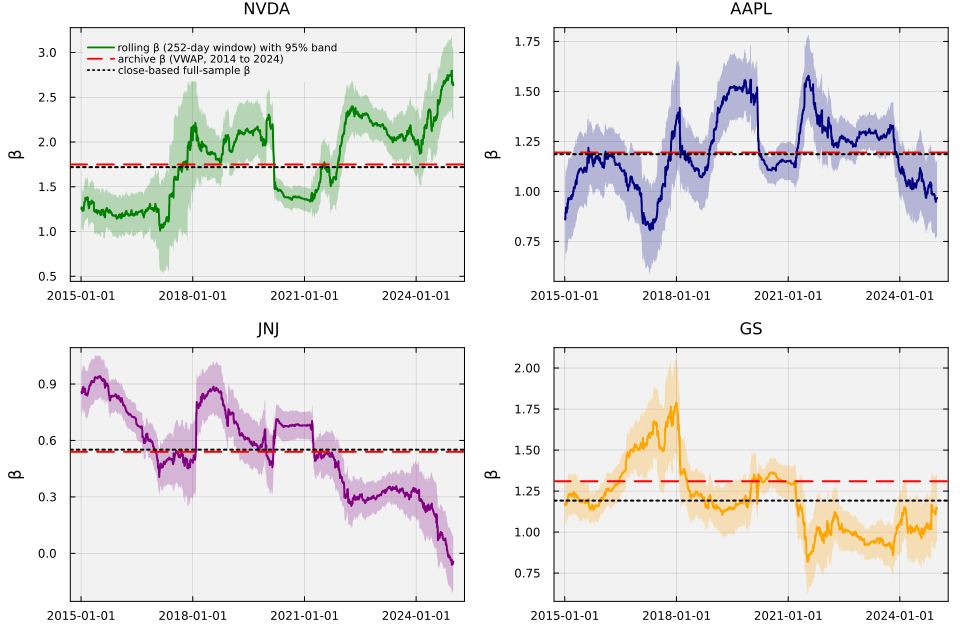
\includegraphics[height=0.50\textheight,keepaspectratio]{../figs/Fig-L7b-Rolling-Beta-Bands.png}
  \end{center}
  \vspace{-0.5em}
  Refit the L6a regression on a one-year window ending on day $t$: $\hat\beta_i(t)$
  with its classical pointwise band $\pm1.96\,\mathrm{SE}$ (descriptive: iid
  assumptions, overlapping windows). It gives the motion a \hilite{scale}: a
  constant beta wanders inside such bands; an excursion of many band-widths
  lasting years would be unusual (NVDA: $1.0$ to $2.8$ against $1.75$).
\end{frame}

\begin{frame}{Why Frozen Parameters Can Fail: The Consequences}
  Rolling bands motivate testing an updating rule; they do not prove drift or
  promise improvement. A moving $(\alpha_i,\beta_i)$ acts on the engine in three
  places:
  \begin{itemize}\setlength{\itemsep}{0.3em}
    \item \hilite{The threshold} $-\alpha_i/\beta_i$: the frozen thresholds sit
      within a few tenths per year of zero, so the basket hangs on whether $\gt$
      is above or below a narrow band; an intercept that moves by a few tenths per
      year moves the threshold by more.
    \item \hilite{The basket and the weights}: the magnitude of $\gamma_i(t)$
      moves through the lens $\beta_i^{\xi_t}$; a non-positive beta breaks the
      lens, so L7a's rule (assign to the non-preferred set) becomes necessary.
    \item \hilite{The covariance matrix} $\SigSIM=s^2_{g,M}\hat{\bbe}\hat{\bbe}^{\top}+\hat{\mathbf D}_g$
      ($\hat{\mathbf D}_g$: residual variances): with $s^2_{g,M}$ held fixed, the online betas and residual scales
      move it by 39\% to 63\% (Frobenius) after the identical first day.
  \end{itemize}
  None of this says updating helps: freezing is a choice with consequences.
\end{frame}

% ==== EWLS ===================================================
\begin{frame}{EWLS: Weights, Loss, Decay Factor, and Half-Life}
  Exponentially weighted least squares keeps the L6a regression and changes the
  weight each day carries. Fix asset $i$; for days $s=1,\ldots,t$ let
  $\bx_s=(1,g_{M,s})^{\top}$, $y_s=g_{i,s}$ (inverse years), $\bth=(\alpha,\beta)^{\top}$.
  Choose a \hilite{half-life} $\thalf>0$ (trading days) and set the \hilite{decay
  factor} $\delta=2^{-1/\thalf}\in(0,1)$, so $\delta^{\thalf}=1/2$. The estimate at
  time $t$ minimizes:
  \[
    \boxed{L_t(\bth)=\sum_{s=1}^{t}\underbrace{\delta^{\,t-s}}_{\text{weight of day }s}
      \bigl(y_s-\bx_s^{\top}\bth\bigr)^2}
  \]
  \begin{itemize}\setlength{\itemsep}{0.2em}
    \item An observation $\thalf$ days old carries half today's weight; the total
      weight of the past is $\sum_{s\le t}\delta^{t-s}\to1/(1-\delta)\approx\thalf/\ln2$,
      about 91 current-observation equivalents for a one-quarter half-life (a
      count of weight, not an effective sample size).
    \item For this data-only loss, ordinary least squares is the case $\delta=1$.
  \end{itemize}
\end{frame}

\begin{frame}{EWLS: Sufficient Statistics and the Recursion}
  \vspace{-0.3em}
  The loss is quadratic, so its minimizer solves a two-by-two system whose
  coefficients are weighted sums over the past, the weighted Gram matrix,
  cross-moment vector, and response second moment:
  \[
    \bA_t=\sum_{s\le t}\delta^{t-s}\bx_s\bx_s^{\top}\in\R^{2\times2},\qquad
    \bb_t=\sum_{s\le t}\delta^{t-s}\bx_s\,y_s\in\R^{2},\qquad
    c_t=\sum_{s\le t}\delta^{t-s}y_s^2
  \]
  $\nabla_{\bth}L_t=\mathbf 0$ gives $\bA_t\bth=\bb_t$. Every weight of day $s$ at
  time $t$ is $\delta$ times its weight at $t-1$, and today enters with weight one,
  so each moment updates in one step:
  \[
    \boxed{\bA_t=\delta\,\bA_{t-1}+\bx_t\bx_t^{\top},\qquad
      \bb_t=\delta\,\bb_{t-1}+\bx_t\,y_t,\qquad
      c_t=\delta\,c_{t-1}+y_t^2}
  \]
  Solve $\bA_t\hat{\bth}_{i,t}=\bb_t$ directly (no inverse); the residual scale
  from the same moments, because the cross term cancels at the optimum:
  \[
    \hat\sigma_{\varepsilon,i,t}=\sqrt{\frac{c_t-\hat{\bth}_{i,t}^{\top}\bb_t}{[\bA_t]_{11}}},
    \qquad [\bA_t]_{11}=\textstyle\sum_{s\le t}\delta^{t-s}\ \text{(total weight; no dof correction)}
  \]
  \vspace{-0.9em}
  Three moments are \hilite{sufficient}: constant memory, constant work per day.
\end{frame}

\begin{frame}{EWLS: The Prior, and the Units}
  \vspace{-0.3em}
  $\bA_0=\mathbf 0$ leaves the first days unidentified. Seed with the archive
  estimate $(\bth_{i,0},\sigma_{\varepsilon,i,0})$ worth $N_0$ pseudo-observations
  through $\bM=\E[\bx\bx^{\top}]=\bigl(\begin{smallmatrix}1&g'_M\\ g'_M&s^2_{g,M}+g'^{2}_M\end{smallmatrix}\bigr)$
  (training market moments):
  \[
    \boxed{\bA_0=N_0\,\bM,\qquad \bb_0=\bA_0\,\bth_{i,0},\qquad
      c_0=\bth_{i,0}^{\top}\bb_0+N_0\,\sigma^2_{\varepsilon,i,0}}
  \]
  \begin{itemize}\setlength{\itemsep}{0.25em}
    \item Returns the prior exactly before any update; after $t$ updates its
      weight is $\delta^tN_0$: it \hilite{decays like the data}. The seeded estimate
      minimizes $L_t(\bth)+\delta^tN_0(\bth-\bth_{i,0})^{\top}\bM(\bth-\bth_{i,0})$
      (advanced notebook); ridge (L6a advanced) is a different modification.
    \item \hilite{Units}: annualized daily growth rates from closes; $\alpha$,
      $\hat\sigma_\varepsilon$ in inverse years, $\beta$ dimensionless, $\delta$ per
      observation, $\thalf$ in trading days, $N_0$ in pseudo-observations. $\bM$ is
      VWAP-based ($4.6$ vs $7.5$ on closes): 63 pseudo-observations carry the
      slope information of about 39 close-based days.
  \end{itemize}
\end{frame}

\begin{frame}{Algorithm: EWLS SIM Update (Online)}
  \textbf{\ink{Initialize:}} the prior for each asset, the archive market moments,
  $N_0$, $\thalf$ (hence $\delta$); seed $(\bA_0,\bb_0,c_0)$, the same $\bA_0$ for
  every asset.

  \vspace{0.3em}
  \textbf{\ink{For each new trading day $t$:}}
  \begin{enumerate}\setlength{\itemsep}{0.15em}
    \item After the close, observe $g_{M,t}$ and $g_{i,t}$ for every asset; form
      $\bx_t=(1,g_{M,t})^{\top}$.
    \item Update every asset's moments: $\bA_t\leftarrow\delta\bA_{t-1}+\bx_t\bx_t^{\top}$,
      $\bb_t\leftarrow\delta\bb_{t-1}+\bx_tg_{i,t}$, $c_t\leftarrow\delta c_{t-1}+g_{i,t}^2$.
    \item Solve $\bA_t\hat{\bth}_{i,t}=\bb_t$ and compute $\hat\sigma_{\varepsilon,i,t}$;
      if numerically unidentified, keep the previous estimate.
    \item Hand $(\hat\alpha_{i,t},\hat\beta_{i,t},\hat\sigma_{\varepsilon,i,t})$ to the
      engine for use on day $t+1$, \hilite{never on day $t$}.
  \end{enumerate}
  \textbf{\ink{Output:}} the parameter paths and the final moments. Package:
  \texttt{ewls\_init}, \texttt{ewls\_update!}, \texttt{ewls\_path}.
  \slidenote{Example 1:}{\dimmed{CHEME-5660-L7b-Example-EWLS-Replay-Fall-2026.ipynb}}
\end{frame}

% ==== replay ================================================
\begin{frame}{Chronological Replay: Declaring the Half-Life}
  The half-life is the one knob, chosen \hilite{inside the training period} by a
  walk-forward comparison: for each $\thalf\in\{21,63,126,252,\infty\}$, run the
  recursion over 2014 to 2024 seeded on the first 252 growth rates alone, and on
  every day $t$ of 2020 to 2024 predict from the parameters through $t-1$:
  \[
    \hat g_{i,t\,|\,t-1}=\hat\alpha_{i,t-1}+\hat\beta_{i,t-1}\,g_{M,t}
    \qquad(\text{conditional on }g_{M,t}\text{: a test, not a forecast})
  \]
  \begin{itemize}\setlength{\itemsep}{0.2em}
    \item One quarter wins on aggregate ($1.9\%$ below no forgetting) and for
      seven of thirteen firms. \hilite{Declared}: $\thalf^\star=63$ trading days;
      nothing re-tunes it. The criterion scores $\hat\alpha+\hat\beta g_M$, not the
      threshold classification the engine acts on.
    \item \hilite{The replay}: frozen reads the archive every day; online restarts
      on the first 2025 day from the archive prior ($N_0=63$), updates on close-based
      growth rates, and on day $t$ reads the parameters that stood \hilite{before}
      day $t$'s observation. Parameters diverge from day 2; trades from day 22.
  \end{itemize}
\end{frame}

\begin{frame}{Chronological Replay: What Changed in 2025}
  \vspace{-0.3em}
  \begin{columns}[T]
    \begin{column}{0.36\textwidth}
      \centering
      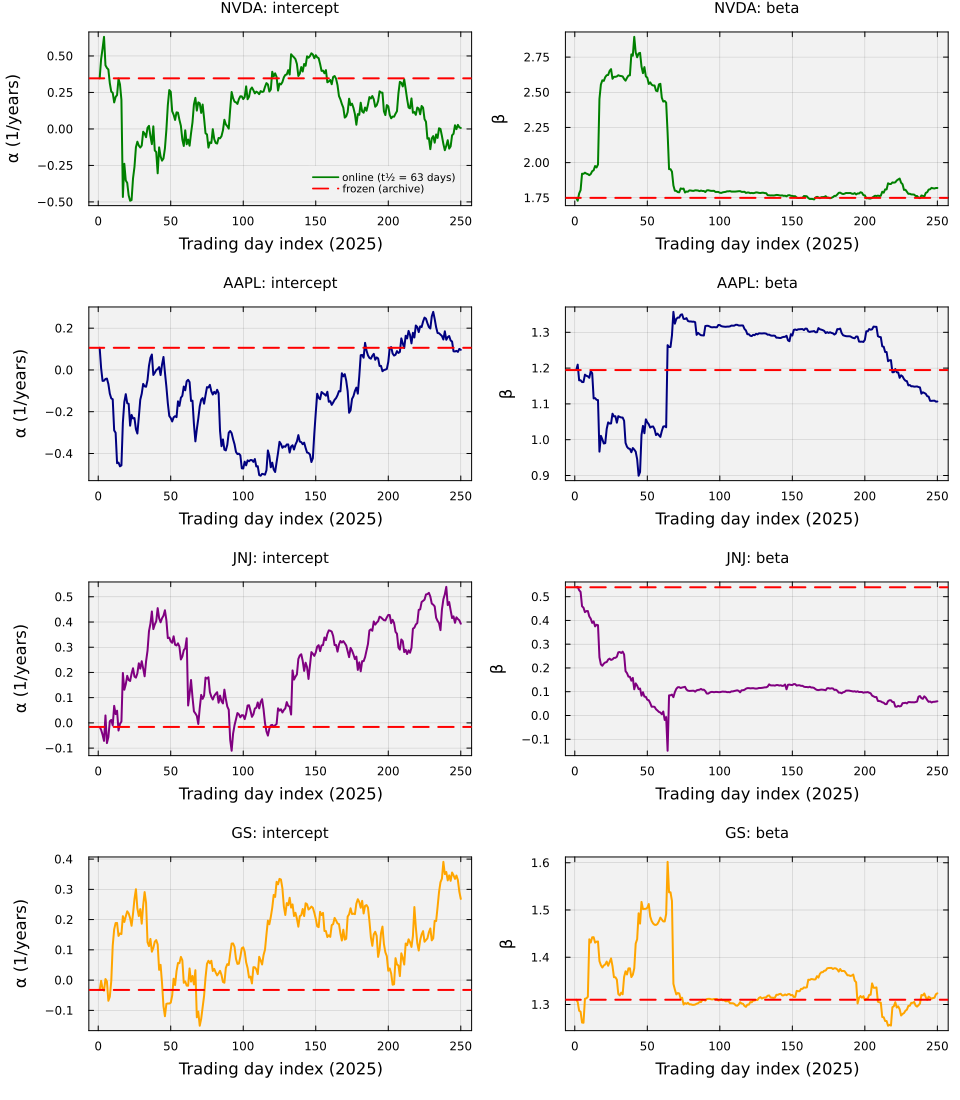
\includegraphics[height=0.62\textheight,keepaspectratio]{../figs/Fig-L7b-Online-Paths-2025.png}
    \end{column}
    \begin{column}{0.64\textwidth}
      \begin{itemize}\setlength{\itemsep}{0.35em}
        \item Online betas moved by half a unit or more, intercepts by several
          tenths per year (the least identified parameter at a one-quarter
          memory); the arms disagreed on at least one firm on 101 of 250 days;
          empty basket 12 days (online) against 57; JNJ's beta non-positive for
          three April days (the rule applied).
        \item \hilite{Updating hurt}: online monthly $1.33$ against frozen $1.53$
          (daily $1.26$ against $1.40$), twice the turnover, one breaker firing.
        \item One draw, not a probability. Where the gap opened: next frame.
      \end{itemize}
    \end{column}
  \end{columns}
  \slidenote{Example 2:}{\dimmed{CHEME-5660-L7b-Example-Scenario-Ensemble-Fall-2026.ipynb}}
\end{frame}

\begin{frame}{Chronological Replay: Two Episodes, One Rerun}
  \vspace{-0.2em}
  Example 2 pins the gap to dates, holdings, and one rerun:
  \begin{itemize}\setlength{\itemsep}{0.25em}
    \item \hilite{Spring}: the online intercept of JNJ put that firm alone into a
      basket the frozen thresholds left empty (98\% of the online book on March 31,
      ahead $3.5\%$); the April fall left the online arm $8.9\%$ down and about 58
      dollars behind, a gap near 40 to 56 dollars until November.
    \item \hilite{November}: both arms peaked on November 12 and drew down to
      November 20, frozen by $9.0\%$, online by $10.1\%$, a tenth over the limit:
      the breaker liquidated the online book, its lock covered the December
      rebalance day, and the book sat in cash to year end.
    \item \hilite{Counterfactual}: breaker disabled, the same online engine ends at
      $1.50$; the firing is 166 of the 202 dollars of the gap.
    \item Not ``the rule, not the estimator'': the estimates changed the holdings,
      the holdings crossed the threshold, the discontinuous rule amplified a tenth
      of a percent into a quarter of a year in cash; one path cannot separate them.
  \end{itemize}
\end{frame}

% ==== ensemble ==============================================
\begin{frame}{The Scenario Ensemble: The SIM Generator}
  \vspace{-0.3em}
  To compare policies across many possible years, draw futures from the model
  the engine carries: from the decision-date closes, for $t=1,\ldots,N$,
  independently across days and assets, in inverse years,
  \[
    \boxed{g_{M,t}\sim\mathcal N\bigl(g'_M,\,s^2_{g,M}\bigr),\qquad
      \varepsilon_{i,t}\sim\mathcal N\bigl(0,\,s^2_{g,\varepsilon,i}\bigr),\qquad
      g_{i,t}=\hat\alpha_i+\hat\beta_i\,g_{M,t}+\varepsilon_{i,t}}
  \]
  then compound with $\Delta t=1/252$ yr: $S_M(t)=S_M(t-1)\,e^{g_{M,t}\Delta t}$,
  $S_i(t)=S_i(t-1)\,e^{g_{i,t}\Delta t}$; the shared draw makes the assets co-move as $\SigSIM$ says.
  \vspace{-0.2em}
  \begin{itemize}\setlength{\itemsep}{0.15em}
    \item \hilite{Units}: draw daily growth rates in annualized units; $\Delta t$
      enters once, in the exponent: a one-day log return with mean $g'_M\Delta t$,
      variance $s^2_{g,M}\Delta t^2$ (L4b, L5a).
    \item \hilite{Scenario engine, not validation}: Gaussian, independent
      residuals, constant parameters, VWAP-smoothed moments; \hilite{same
      generator} (L5b): the frozen parameters are the generator's own, so online
      estimates track noise; the benefit under drift is out of reach.
  \end{itemize}
\end{frame}

\begin{frame}{The Scenario Ensemble: The Distributional Scorecard}
  With $n$ futures of $N$ days ($T=N\Delta t$; $\WP$ the account's wealth, $g_f$
  the risk-free rate), terminal wealths sorted $W_{(1)}\le\cdots\le W_{(n)}$,
  drawdowns $D^{(p)}$, tail level $5\%$, $k=\lceil0.05\,n\rceil$:
  \begin{itemize}\setlength{\itemsep}{0.12em}
    \item \hilite{Median terminal wealth, median NPV}: the typical outcome; did it
      beat cash at $g_f$.
    \item \hilite{Fail rate}: fraction of futures with $W^{(p)}_{\mathcal P}(T)<\WP(0)e^{g_fT}$
      (negative NPV).
    \item \hilite{Lower quantile at 5\%}: the order statistic $W_{(k)}$, so at
      least 5\% of futures end at or below it (with $n=2000$: the hundredth
      smallest, a definite number).
    \item \hilite{Tail mean at 5\%}: $\frac1k\sum_{j\le k}W_{(j)}$, the worst 5\%
      on average.
    \item \hilite{Drawdown median and 5\% upper cutoff}: the median and the
      $k$-th largest $D^{(p)}$.
  \end{itemize}
  \hilite{Paired}: both arms run on the same futures, so compare online minus
  frozen terminal wealth per future (median, spread, fraction positive); pairing
  holds the draws fixed and leaves the policy contrast.
\end{frame}

\begin{frame}{The Scenario Ensemble: Two Thousand Futures}
  \vspace{-0.3em}
  \begin{columns}[T]
    \begin{column}{0.42\textwidth}
      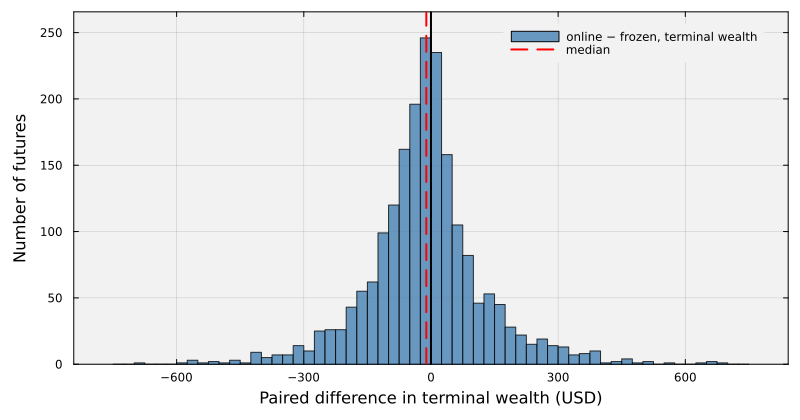
\includegraphics[width=\textwidth]{../figs/Fig-L7b-Paired-Differences.png}
    \end{column}
    \begin{column}{0.58\textwidth}
      \begin{itemize}\setlength{\itemsep}{0.25em}
        \item \hilite{Frozen, monthly}: median $1.14$ times initial wealth, fail
          rate $27\%$, 5\% quantile $0.93$, tail mean $0.89$, median drawdown
          $10.6\%$. The realized 2025 ($1.53$) was a favorable draw.
        \item \hilite{Online, monthly}: a little worse on every column (median
          $1.12$, fail $31\%$, quantile $0.90$); SPY is close to both.
        \item \hilite{Paired}: median about $-11$ on a thousand, standard deviation
          about $140$; online ahead on $44\%$ of futures, below half: the observed
          cost of updating with no drift to learn.
      \end{itemize}
    \end{column}
  \end{columns}
  \slidenote{Example 2:}{\dimmed{CHEME-5660-L7b-Example-Scenario-Ensemble-Fall-2026.ipynb}}
\end{frame}

% ==== gates ==================================================
\begin{frame}{Validation Gates: A Pointer}
  \vspace{0.6em}
  The comparisons of today, frozen against online on a realized path and on an
  ensemble, become in L15a a set of \hilite{deployment gates}: pass-or-fail rules
  with stated limits (a median terminal wealth that must beat the frozen
  baseline, a fail rate and a tail that must not exceed set values, a drawdown
  and a turnover budget), evaluated on the same paired ensemble and reported
  before an online engine is allowed to replace its frozen ancestor.

  \vspace{0.8em}
  Nothing today is such a gate; L15a turns these comparisons into pass or fail.
\end{frame}

% ==== optional advanced material =============================
\begin{frame}{Optional Advanced Material}
  \vspace{0.4em}
  {\normalsize\textbf{\ink{Advanced:}} \dimmed{advanced/online\_learning/}\par
  \dimmed{CHEME-5660-L7b-Advanced-EWLS-Recursion-Fall-2026.ipynb}}

  \vspace{0.7em}
  Optional, not a prerequisite for L8b. Derives the weighted normal equations
  and the three sufficient statistics from the exponentially weighted loss,
  shows the one-step recursion, solves for the parameters and the residual scale
  (with the cancellation that makes the residual formula work), and proves that
  the prior seeding returns the prior exactly and that the seeded recursion
  minimizes the data loss plus a decaying prior-centered quadratic.
  \slidenote{Notebook:}{\href{https://github.com/varnerlab/CHEME-5660-CourseRepository-Fall-2026/tree/main/lectures/week-7/L7b/advanced}{lectures/week-7/L7b/advanced}, also linked from the lecture notebook.}
\end{frame}

\begin{frame}{Summary}
  Today: pooled parameters that mask time variation; the EWLS recursion; a replay
  under a declared half-life; a SIM scenario ensemble and its scorecard.

  {\large\textbf{\ink{Key takeaways}}}
  \begin{itemize}\setlength{\itemsep}{0.1em}
    \item \hilite{A frozen parameter is a modeling choice, and rolling bands give
      the motion a scale}: a moving intercept or beta moves the threshold, the
      basket, and the SIM covariance.
    \item \hilite{EWLS is least squares with a memory, and everything about it is
      stated}: decay and half-life, sufficient moments, a two-by-two solve, a prior
      that decays like the data, a half-life chosen inside the training period.
    \item \hilite{Compare policies on many futures, and say what the futures are}:
      on 2025 the online engine finished behind, mostly through one breaker firing;
      on two thousand futures the frozen engine's typical outcome was far below its
      2025 result and online paid a small price with no drift to learn; not validation.
  \end{itemize}
  Next, L8b: option contracts. Frozen versus online returns in L15a as gates.
\end{frame}

\transitionframe{Today: parameters that move, an estimator that forgets at a stated rate, and a scorecard read across many futures.}

\end{document}
